\chapter{Introduction}
\section{Language Server Protocol}
Language server protocol announced in 2016 \cite{language-server-protocol:2016},
and it allows software engineers to implement only one piece of software that
can interact with several IDEs and text editors solving the $M \times N$
problem, where $M$ is the number of programming languages that require `language
intelligence' support and $N$ is the number of text editors that can provide
such support. 

\begin{figure}[hbt]
\centering
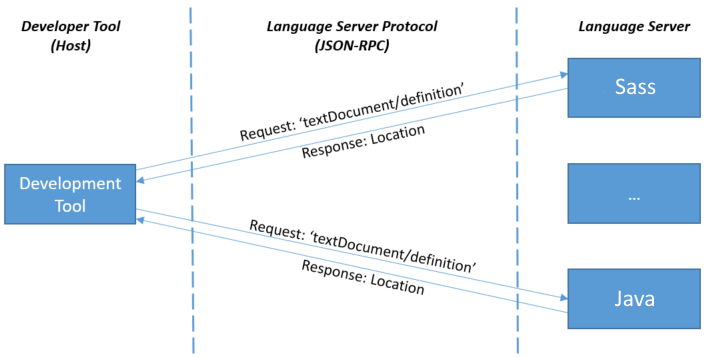
\includegraphics[width=0.7\textwidth]{figs/language-server.png}

\caption{The schematic represents interaction between IDE and different language
servers \cite{language-server-protocol:2016}}

\label{fig:lsp-language-editors}
\end{figure} 

The protocol itself consists of JSON-RPC 2.0 \cite{jsonrpc:2010} messages
representing different kinds of requests and notifications from both client and
server. It is not necessary for a language server developert to support all
features defined in the protocol. For example, one can only implement the type
ascription ($\texttt{textDocument/hover}$) and `Goto definition'
($\texttt{textDocument/definition}$) capabilities. Below is an example of
communication between language server and the client. The protocol itself does
not define a specific transport that the developers must use to communicate with
the server. The communication might be implemented through the API calls, using
IPC (Inter Process Communication) as a separate running binaries or even through
the network.

\begin{figure}[hbt]
\centering
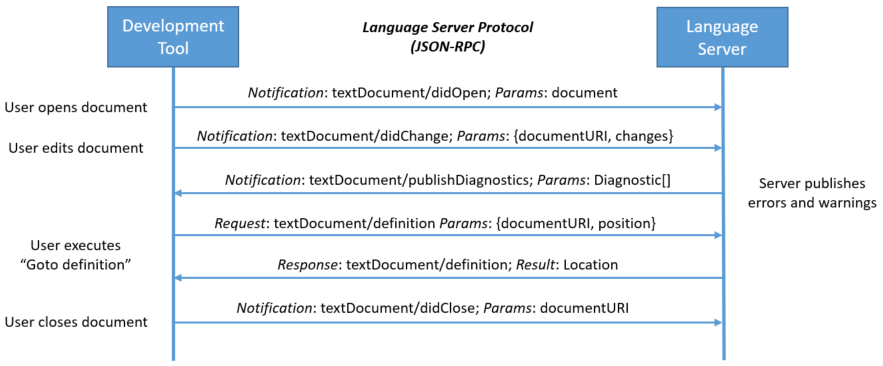
\includegraphics[width=0.9\textwidth]{figs/language-server-sequence.png}

\caption{Routine communication between language server and development tool
\cite{language-server-protocol:2016}}

\label{fig:lsp-routine-communication}
\end{figure} 

\section{Jasmin programming language}

Cryptographic software plays a crucial role in modern software development.
Although it typically constitutes only a small part of the overall codebase,
it often covers the most critical security functions, e.g. the
OpenSSL library implements the SSL/TLS protocols, which are fundamental to
securing the vast majority of internet communications.  

Serious vulnerabilities in cryptographic software show how crritical it is. For
example, the Heartbleed \cite{heartbleed:2014} vulnerability (CVE-2014-0160),
which was publicly disclosed in 2014. This flaw affected systems running
vulnerable versions of OpenSSL, allowing attackers to read server memory. As a
result, private keys used for traffic encryption could be exposed, allowing an
attacker to access unencrypted HTTPS traffic.

To lower the risks of implementation vulnerabilities, researchers have developed
programming frameworks that enable formal verification of cryptographic
primitives against attacks. One such framework is Jasmin
\cite{jasmin:2017}. 

Jsamin is a cryptographic framework designed for implementing cryptographic 
primitives, such as hash functions or digital signature schemes. One of the 
recent studies~\cite{jasmin-sha3:2019} showed its applicability for modern 
cryptographic primitives.

Additionally, Jasmin compiler allows for the transpilation of Jasmin source code
into EasyCrypt \cite{easycrypt:2013} specifications for further
formal verification of security properties.

This work focuses primarily on the Jasmin language itself, particularly, the
language server implementation for the Jasmin language.

\section{Contribution}

In this work, we report the progress in implementing a language server
infrastructure for the Jasmin  programming language. 

The principal contributions of this research include the implementation of a
language server for the Jasmin programming language, which has:

\begin{itemize}
    \item Diagnostics support for the Jasmin language
    \item Goto definition support ($\texttt{textDocument/definition}$)
    \item Reference highlight support ($\texttt{textDocument/highlight}$)
    \item Type ascription support ($\texttt{textDocument/hover}$)
    \item Tree-sitter support for the Jasmin language
\end{itemize}
